\documentclass{beamer}

\usepackage{tikz}
\usepackage{pdfpages}
\usetikzlibrary{shapes,snakes}

\newcommand{\smtc}[1]{\texttt{#1}}
\newcommand{\smtcuc}[1]{\texttt{\color{blue}#1}}
\newcommand{\tdots}{$...$}

% switch off the fancy navigation symbols
\setbeamertemplate{navigation symbols}{}

\title[SMT-COMP 2018]{${}$\\[3.5em]13th International\\
Satisfiability Modulo Theories\\
Competition\\[.7em]
SMT-COMP 2018\\[3em]}

\author{Matthias Heizmann \and Aina Niemetz\\ \and Giles Reger \and
  \underline{Tjark Weber}}

\institute{}

\date{}

\logo{\vspace{2.7cm}\includegraphics[width=\textwidth]{laurels}\hspace{.8cm}}

\begin{document}

%%%%%%%%%%%%%%%%%%%%%%%%%%%%%%%%%%%%%%%%%%%%%%%%%%%%%%%%%%%%%%%%%%%%%%%%%%%%%%%%

\frame{\titlepage}
\logo{}

%%%%%%%%%%%%%%%%%%%%%%%%%%%%%%%%%%%%%%%%%%%%%%%%%%%%%%%%%%%%%%%%%%%%%%%%%%%%%%%%

\section{}% leave this empty
\subsection{}% leave this empty

%%%%%%%%%%%%%%%%%%%%%%%%%%%%%%%%%%%%%%%%%%%%%%%%%%%%%%%%%%%%%%%%%%%%%%%%%%%%%%%%

\begin{frame}{Background}
  SMT-COMP is an annual competition between SMT solvers.  It was first
  held in 2005.

  \bigskip
  \bigskip

  \begin{center}
    Satisfiability Modulo Theories =

    \medskip
    
    propositional satisfiability + background theories (+ quantifiers)
  \end{center}
\end{frame}

%%%%%%%%%%%%%%%%%%%%%%%%%%%%%%%%%%%%%%%%%%%%%%%%%%%%%%%%%%%%%%%%%%%%%%%%%%%%%%%%

\begin{frame}{Solvers, Logics, and Benchmarks}
  \begin{itemize}
  \item 17 teams participated
    \smallskip
  \item Solvers:\\
    \smallskip
    \usebeamercolor{structure}
    \begin{tikzpicture}
      \draw (0,-.25) -- (0,1.25);
      \node [left] at (0,1) {\footnotesize Main track};
      \node [left] at (0,.5) {\footnotesize Application track};
      \node [left] at (0,0) {\footnotesize Unsat-core track};

      \draw [fill=fg] (0,.85) rectangle (3,1.15);
      \node [left,white] at (3,1) {\footnotesize 20};
      \draw [fill=fg!30!white] (3,.85) rectangle (3.6,1.15);
      \node [right] at (3.6,1) {\tiny 4 non-competing};

      \draw [fill=green!80!black] (0,.35) rectangle (0.6,.65);
      \node [left] at (0.6,.5) {\footnotesize 4};
      \draw [fill=green!30!white] (0.6,.35) rectangle (0.9,.65);
      \node [right] at (0.9,.5) {\tiny 2 non-competing};

      \draw [fill=yellow!80!red] (0,-.15) rectangle (.45,.15);
      \node [left] at (.45,0) {\footnotesize 3};
      \draw [fill=yellow!30!white] (.45,-.15) rectangle (.75,.15);
      \node [right] at (.75,0) {\tiny 2 non-competing};
    \end{tikzpicture}
  \item Logics:\\
    \smallskip
    \begin{tikzpicture}
      \draw (0,-.25) -- (0,1.25);
      \node [left] at (0,1) {\footnotesize Main track};
      \node [left] at (0,.5) {\footnotesize Application track};
      \node [left] at (0,0) {\footnotesize Unsat-core track};

      \draw [fill=fg] (0,.85) rectangle (4.9,1.15);
      \node [left,white] at (4.9,1) {\footnotesize 49};
      \draw [fill=fg!30!white] (4.9,.85) rectangle (5,1.15);
      \node [right] at (5,1) {\tiny 1 experimental};

      \draw [fill=green!80!black] (0,.35) rectangle (2.1,.65);
      \node [left] at (2.1,.5) {\footnotesize 21};

      \draw [fill=yellow!80!red] (0,-.15) rectangle (4.4,.15);
      \node [left] at (4.4,0) {\footnotesize 44};
    \end{tikzpicture}
  \item Benchmarks:\\
    \smallskip
    \begin{tikzpicture}
      \draw (0,-.25) -- (0,1.25);
      \node [left] at (0,1) {\footnotesize Main track};
      \node [left] at (0,.5) {\footnotesize Application track};
      \node [left] at (0,0) {\footnotesize Unsat-core track};

      \draw [fill=fg] (0,.85) rectangle (6.66482,1.15);
      \node [left,white] at (6.66482,1) {\footnotesize 333241};

      \draw [fill=green!80!black] (0,.35) rectangle (0.18514,.65);
      \node [right] at (0.18514,.5) {\footnotesize 9257};

      \draw [fill=yellow!80!red] (0,-.15) rectangle (2.6141,.15);
      \node [left] at (2.6141,0) {\footnotesize 130705};

    \end{tikzpicture}
  \end{itemize}
\end{frame}

%%%%%%%%%%%%%%%%%%%%%%%%%%%%%%%%%%%%%%%%%%%%%%%%%%%%%%%%%%%%%%%%%%%%%%%%%%%%%%%%

\begin{frame}{Job Pairs}
  \medskip

  \structure{1,776,062} job pairs {\footnotesize (+ some repeats)}; over \structure{11 years} of processor time

  \begin{center}
    \usebeamercolor{structure}
    \begin{tikzpicture}
      \draw [gray] (0,0) -- (10,0);
      \draw [gray] (0,.9) -- (10,.9);
      \draw [gray] (0,1.8) -- (10,1.8);
      \draw [gray] (0,2.7) -- (10,2.7);
      \draw [gray] (0,3.6) -- (10,3.6);
      \draw [gray] (0,4.5) -- (10,4.5);
      \draw [gray] (0,5.4) -- (10,5.4);

      \node [left,gray] at (0,0) {\tiny 0};
      \node [left,gray] at (0,.9) {\tiny 300,000};
      \node [left,gray] at (0,1.8) {\tiny 600,000};
      \node [left,gray] at (0,2.7) {\tiny 900,000};
      \node [left,gray] at (0,3.6) {\tiny 1,200,000};
      \node [left,gray] at (0,4.5) {\tiny 1,500,000};
      \node [left,gray] at (0,5.4) {\tiny 1,800,000};

      \draw [fill=lightgray] (1,0) rectangle (2,1.019142);
      \draw [fill=lightgray] (2.75,0) rectangle (3.75,3.085845);
      \draw [fill=lightgray] (4.5,0) rectangle (5.5,4.687632);
      \draw [fill=lightgray] (6.25,0) rectangle (7.25,4.366839);
      \draw [fill=fg] (8,0) rectangle (9,4.164573);
      \draw [fill=green!80!black] (8,4.164573) rectangle (9,4.277862);
      \draw [fill=yellow!80!red] (8,4.277862) rectangle (9,5.328186);

      \node [white] at (8.5,2.0822865) {\footnotesize Main};
      \node [] at (9.4,4.2212175) {\footnotesize App};
      \node [] at (8.5,4.7463795) {\footnotesize UC};

      \node [below,gray] at (1.5,0) {\footnotesize 2014};
      \node [below,gray] at (3.25,0) {\footnotesize 2015};
      \node [below,gray] at (5,0) {\footnotesize 2016};
      \node [below,gray] at (6.75,0) {\footnotesize 2017};
      \node [below] at (8.5,0) {\footnotesize 2018};
    \end{tikzpicture}
  \end{center}
\end{frame}

%%%%%%%%%%%%%%%%%%%%%%%%%%%%%%%%%%%%%%%%%%%%%%%%%%%%%%%%%%%%%%%%%%%%%%%%%%%%%%%%

\begin{frame}{}
  \begin{center}
    \vfill
      {\huge \structure{Selected Results}}
    \vfill
  \end{center}
\end{frame}

%%%%%%%%%%%%%%%%%%%%%%%%%%%%%%%%%%%%%%%%%%%%%%%%%%%%%%%%%%%%%%%%%%%%%%%%%%%%%%%%

\begin{frame}{Unsat-Core Track}
  \begin{itemize}
  \item 3 competing solvers: CVC4, SMTInterpol, Yices-2.6.0
  \item 16 competitive divisions (out of 44)
  \end{itemize}

  \bigskip

  \begin{center}
    \begin{tabular}{lp{.7\textwidth}}
    Solver      & Divisions won \\ \hline \\[-1.5ex]
    CVC4        & QF\_AUFLIA, QF\_IDL, QF\_LIRA, QF\_RDL, QF\_UF \\
    \\[-1.5ex]
    SMTInterpol & QF\_LIA, QF\_LRA, QF\_UFLIA \\
    \\[-1.5ex]
    Yices-2.6.0 & QF\_ABV, QF\_ALIA, QF\_AUFBV, QF\_AX, QF\_BV, QF\_UFBV, QF\_UFIDL, QF\_UFLRA
    \end{tabular}
  \end{center}

  \vspace{-1.6cm}

  \pause
  
  
\begin{tikzpicture}
    \node[draw=red, fill=none, line width=1mm] {
      \begin{minipage}{\textwidth}
        ${}$\\
        ${}$\\
      \end{minipage}
    };
  \end{tikzpicture}
\end{frame}

%%%%%%%%%%%%%%%%%%%%%%%%%%%%%%%%%%%%%%%%%%%%%%%%%%%%%%%%%%%%%%%%%%%%%%%%%%%%%%%%

\begin{frame}{Application Track}
  \begin{itemize}
  \item 4 competing solvers: Boolector, CVC4, SMTInterpol, Yices-2.6.0
  \item 12 competitive divisions (out of 21)
  \end{itemize}

  \bigskip

  \begin{center}
    \begin{tabular}{lp{.7\textwidth}}
      Solver      & Divisions won \\ \hline \\[-1.5ex]
      Boolector   & QF\_ABV, QF\_UFBV\\
      \\[-1.5ex]
      CVC4        & QF\_NIA, QF\_UFNIA\\
      \\[-1.5ex]
      SMTInterpol & QF\_ALIA, QF\_UFLIA\\
      \\[-1.5ex]
      Yices-2.6.0 & QF\_AUFBV, QF\_AUFLIA, QF\_BV, QF\_LIA, QF\_LRA, QF\_UFLRA\\
    \end{tabular}
  \end{center}

  \vspace{-1.6cm}

  \pause
  
  
\begin{tikzpicture}
    \node[draw=red, fill=none, line width=1mm] {
      \begin{minipage}{\textwidth}
        ${}$\\
        ${}$\\
      \end{minipage}
    };
  \end{tikzpicture}  
\end{frame}

%%%%%%%%%%%%%%%%%%%%%%%%%%%%%%%%%%%%%%%%%%%%%%%%%%%%%%%%%%%%%%%%%%%%%%%%%%%%%%%%

\begin{frame}{Main Track}
  \begin{itemize}
  \item 20 competing solvers
  \item 41 competitive divisions (out of 50)
  \end{itemize}

  \vspace{-.5cm}
  
  \begin{center}
    \begin{tabular}{lp{.7\textwidth}}
      Solver        & Divisions won \\ \hline
      Boolector     & {\small QF\_ABV, QF\_BV$^\text{seq}$, QF\_UFBV}\\
      COLIBRI       & {\small QF\_FP}\\
      CVC4          & {\small ALIA, AUFDTLIA, AUFLIA, AUFLIRA, AUFNIRA, BV, LIA, LRA, NIA, QF\_ABVFP, QF\_AUFBV, QF\_BVFP, QF\_LRA, QF\_NIA, UF$^\text{seq}$, UFDT, UFDTLIA, UFIDL, UFLIA, UFLRA}\\
      Minkeyrink-MT & {\small QF\_BV$^\text{par}$}\\
      SMTRAT        & {\small QF\_NIRA}\\
      SPASS-SATT    & {\small QF\_LIA}\\
      Vampire       & {\small NRA, UF$^\text{par}$, UFNIA}\\
      Yices-2.6.0   & {\small QF\_ALIA, QF\_AUFLIA, QF\_AX, QF\_IDL, QF\_LIRA, QF\_NRA, QF\_RDL, QF\_UF, QF\_UFIDL, QF\_UFLIA, QF\_UFLRA, QF\_UFNIA, QF\_UFNRA}
    \end{tabular}
  \end{center}

  \vspace{-6.75cm}

  \pause
  
  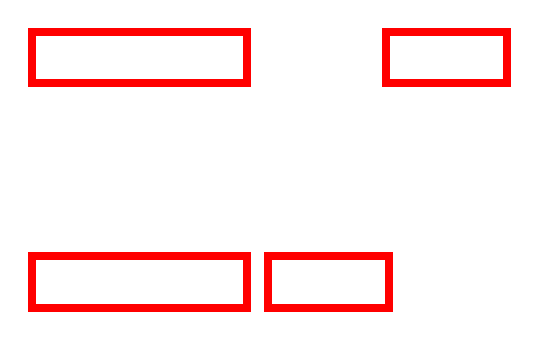
\begin{tikzpicture}
    \node[draw=red, fill=none, line width=1mm] at (0,0) {
      \begin{minipage}{2.5cm}
        ${}$\\
      \end{minipage}
    };
    \node[draw=red, fill=none, line width=1mm] at (2.4,0) {
      \begin{minipage}{1.3cm}
        ${}$\\
      \end{minipage}
    };
    \node[draw=red, fill=none, line width=1mm] at (0,2.85) {
      \begin{minipage}{2.5cm}
        ${}$\\
      \end{minipage}
    };
    \node[draw=red, fill=none, line width=1mm] at (3.9,2.85) {
      \begin{minipage}{1.3cm}
        ${}$\\
      \end{minipage}
    };
  \end{tikzpicture}

  \vspace{3.2cm}
 
\end{frame}

%%%%%%%%%%%%%%%%%%%%%%%%%%%%%%%%%%%%%%%%%%%%%%%%%%%%%%%%%%%%%%%%%%%%%%%%%%%%%%%%

\begin{frame}{Main Track: Competition-Wide Scoring}
  \begin{tabular}{llrr}
                 Rank & Solver & Score (sequential) & Score (parallel)\\ \hline \\[-1.8ex]
    \uncover<5->{1    & CVC4   & 211.99             & 211.99} \\
    \uncover<4->{     & \textcolor{gray}{Z3} & \textcolor{gray}{186.19} & \textcolor{gray}{186.19}} \\
    \uncover<3->{2    & Yices-2.6.0 & 115.26 & 115.26} \\
    \uncover<2->{3    & SMTInterpol &  65.32 &  65.38} \\
    \\
    \multicolumn{4}{l}{Best newcomer:}\\
    7    & SPASS-SATT  &  14.81 &  14.81
  \end{tabular}

  \vspace{-3.6cm}
  
  \uncover<6->{
\begin{tikzpicture}
    \node[draw=red, fill=none, line width=1mm] at (0,0) {
      \begin{minipage}{\textwidth}
        ${}$\\
        ${}$\\
      \end{minipage}
    };
    \node[draw=red, fill=none, line width=1mm] at (0,1.2) {
      \begin{minipage}{\textwidth}
        ${}$\\
      \end{minipage}
    };
  \end{tikzpicture}}

  \vspace{3cm}

\end{frame}

%%%%%%%%%%%%%%%%%%%%%%%%%%%%%%%%%%%%%%%%%%%%%%%%%%%%%%%%%%%%%%%%%%%%%%%%%%%%%%%%

\end{document}

%%%%%%%%%%%%%%%%%%%%%%%%%%%%%%%%%%%%%%%%%%%%%%%%%%%%%%%%%%%%%%%%%%%%%%%%%%%%%%%%

% Local Variables:
% ispell-local-dictionary: "american"
% mode: LaTeX
% mode: flyspell
% LocalWords: curation logics satisfiability Tjark
% End:
